\documentclass{article}

\usepackage[utf8]{inputenc}
\usepackage{graphicx}
\usepackage{listings}
\lstset{language=C++}
\usepackage{hyperref}
\usepackage{amsthm}
\usepackage{amsfonts}
\usepackage{lscape}
\usepackage{multirow}

\theoremstyle{remark}
\newtheorem{tutorial}{Tutorial }

\title{{\tt vle.discrete-time} : simulation of 
recurrent relations into VLE.}

%%%%%%%%%%%%
\begin{document}

\maketitle

\tableofcontents

%%%%%%%%%%%%
\section{Introduction}

The package {\tt record.difference-equation} provides DEVS models
into VLE that allow the simulation of recurrent relations.

This package is intended to be an improvment of difference-equation 
(package {\tt vle.extension.difference-equation}). Improvments are :
\begin{itemize}
  \item there is no propagation of the perturbation
  \item there is no initialization process of the dynamics
  \item it provides Vector of variables.
\end{itemize}

%%%%%%%%%%%%%%%
\section{User Documentation}

%%%%%%%%%%%%%%%
\subsection{Atomic model interface}
\label{sec:user:atomic}

\begin{figure}[!h]
\begin{center} 
\includegraphics[scale=0.80]{figures/userInterface.pdf}
\caption{\label{fig:userInt} The user interface of an atomic model.}
\end{center}
\end{figure}

Evolution of state variables $V_i$ is described by differential equation. 
These expressions can rely on the value of external variables $E_i$.
For time sclicing methods, external variables $E_i$  are expected to be
piecewise constant functions computed from continuous and derivable functions. 
For QSS2, external variables are expected to be
piecewise linear functions.

Atomic model ports $E_i$ and $V_i$ can carry data at time $t$ that contain:
\begin{itemize}
  \item 'name': the name of the external variable (or state variable)
  \item 'value': this is the value at $t$ of the variable 'name'.
  \item 'gradient' (optionnal): this is the value of the gradient of
  the variable 'name' at $t$.
  \item 'discontinuities' (the structure proposed in
  section \ref{sec:theory:strategy}): this should not be handled by the user.
\end{itemize} 
No other assumption, than continuity and derivability of the producing
function, is made regarding external variables updates. Particularly, updates of
$E_i$ variables can occur at any time.

%%%%%%%%%%%%
\subsection{Writing recurrent relations atomic models}
\label{sec:user:diff}

Below is given an example of dynamic for an atomic model that relies 
on the {\tt record.difference-equation}.

\begin{lstlisting}
class MyModel : public DifferenceEquation
{
public:
 MyModel(const DynamicsInit& model,
	     const InitEventList& events) :
    DifferentialEquation(model,events)
 {
 	//Initialisation of variables is done 
 	//into the class constructor:
	v = createVar("v");
	e = createVar("e");
 }
 
 //gradients of state variables are expressed 
 //into the 'compute' function 
 void compute(const Time& time)
 {
    	v =  e(-1) + e(-2) + 0.5;
 }
 //states and external variables are attributes of the class
 Var v;
 Var e;
};
\end{lstlisting}

%%%%%%%%%%%%
\subsection{Configuring atomics models into {\tt vpz} conditions}
\label{sec:user:conf}

The common structure of the conditions for configuring atomic models is the
following:

\begin{itemize}
  \item 'time\_step' (double, default 1.0) : the time step between two
  computing and outputs steps.
  \item init\_value\_myvar (vle::Value, default vle::Double(0.0)) :
  this options designates the initial value of the internal variable 'myvar'.
  It also contains the historic values if $history\_size\_myvar > 0$ using e.g.
  vv::Set.
  \item 'sync\_myvar' (uint, default 0): if $> 0$, the value of 'myvar' 
  at times $n * sync\_myvar * time\_step, \forall n \in \mathbb{N}_+$ is
  expected to be provided by an external event before calling the 'compute'
  function.
  \item 'keep\_first\_value\_myvar' (bool, default false): the first
  value set for 'myvar' at a given time is kept. The following updates for
  'myvar' at this time are ignored.
  \item 'history\_size\_myvar' (uint, default 1) : it gives the size of the
  history of internal variable 'myvar'. 
  \item 'no\_sync\_error\_myvar' (bool, default false) : if true, the access to
  'myvar' at the current time  myvar() will send an error if the last
  time of update of 'myvar' is before the current time.
  \item 'generic' (bool, default true) : if true, all input ports are
  declared as internal variables. Otherwise, internal variables have to be
  declared explicitely using {\tt createVar} c++ functions.
  \item 'all\_sync' (bool, default false) : if true, all internal variables 
  are synchronous. Note that option 'sync\_<myvar>' has priority on 'all\_sync'.
  \item 'bags\_to\_eat' (int, default 0) : the number of bags to wait before
  computing the values of variables (calls of {\tt compute} user function).
\end{itemize} 

%%%%%%%%%%%%
\section{Technical details}

%%%%%%%%%%%%
\subsection{Global architecture}
\label{sec:archi}

\begin{landscape}
\vspace{-10cm}
\begin{figure}[!h]
\begin{center} 
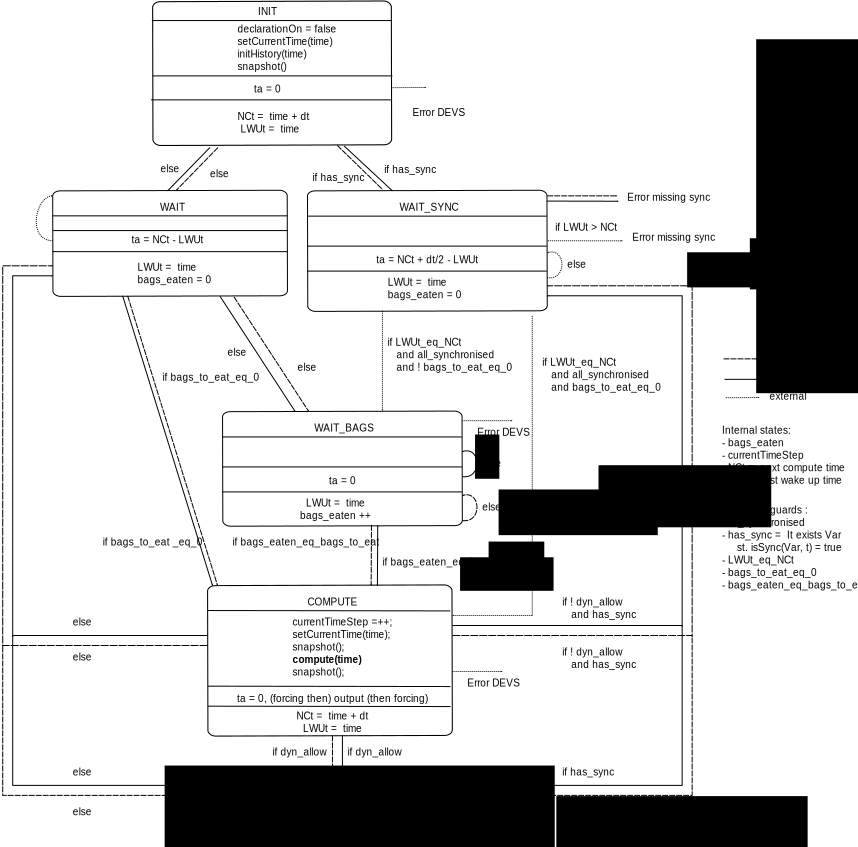
\includegraphics[scale=0.50]{figures/DEVS_states.pdf}
\caption{\label{fig:DEVSgraph} The DEVS state transition graph 
for recurrent relations.}
\end{center}
\end{figure}
\end{landscape}

%%%%%%%%%%%%
\subsection{Simulation time profiling}

Simulation time comparisons are based on the simulation of the Lotka Volterra
model and concern the three softwares VLE, powerdevs and R package deSolve. 
End time of simulation is set to 1500.
Two integration schemes are tested:
\begin{itemize}
  \item RK4 scheme with a time step of 0.01 (for deSolve and VLE)
  \item QSS2 scheme with a quantum value of 0.0001 (for powerdevs and VLE). Note
  that a lower quantum value results in a divergence process (and a $ta \to
  0$).
\end{itemize}
Different observations schemes are tested:
\begin{itemize}
  \item For VLE and powerdevs. A null observation which provides no output
  data.
  \item For VLE. A timed observation with a time-step of 0.01 and a 
  storage into a file.
  \item For VLE. A timed observation with a time-step of 0.01 and a 
  storage into memory. At the beginning, the matrix contains 
  10000 rows and is updated with 10000 more rows each time it is required to
  enlarge the matrix (these are the maximal values for VLE).
  \item For deSolve. A timed observation with a time-step of 0.01 and a 
  storage into a R matrix.
  \item For powerdevs. A plot using gnuplot of quantized values.
\end{itemize}


% \begin{tabular}{|c|c|c|c|}
% ~ & ~ & ~ & ~ \\
% \end{tabular}
\begin{figure}
\begin{center}
\begin{tabular}{|c|c|c|c|}
\hline
soft                      & observation         & RK4     & QSS2  \\\hline\hline
\multirow{2}{*}{powerdevs}& gnuplot             &  -      & 3.86  \\ \cline{2-4}
                          & null                &  -      & 0.76**  \\ \hline
deSolve                   & timed, mem. storage &  14.776* & -     \\ \hline
\multirow{3}{*}{VLE}      & timed, mem. storage &  6.468*  & 10.536\\\cline{2-4} 
                          & timed, file storage &  3.468  & 7.812 \\ \cline{2-4}
                          & null                &  1.072  & 4.824** \\ \hline
\end{tabular}
\caption{Comparison of time executions given in seconds.}
\end{center}
\end{figure}

%\bibliographystyle{plain}
%\bibliography{biblio}


\end{document}